
%(BEGIN_QUESTION)
% Copyright 2006, Tony R. Kuphaldt, released under the Creative Commons Attribution License (v 1.0)
% This means you may do almost anything with this work of mine, so long as you give me proper credit

Lag ditt eget dimensjoneringsproblem for ventil med gitt stromningsrate, spesifikk vekt (densitet) for vaeske, oppstroms- og nedstromstrykk, og en faktisk reguleringsventil spesifisert fra en produsents produktmanual (f.eks. Fisher ``E'' body globe valve product bulletin, eller tilsvarende).  Basert de gitte variablene i problemet ditt pa folgende diagram, og anta turbulent vaeskestrom (ingen choked flow-forhold eller annen raritet som krever en ikke-standard stromningligning):

$$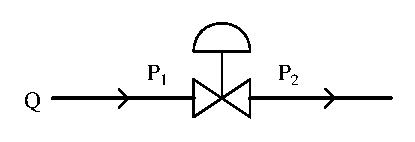
\includegraphics[width=15.5cm]{i00065x01.eps}$$

\begin{itemize}
\item{} {\bf Gitte forhold}
\vskip 5pt 
\item{} Stromningsrate $Q$ =
\vskip 5pt 
\item{} Spesifikk vekt for vaeske $G_f$ = 
\vskip 5pt 
\item{} Oppstromstrykk $P_1$ ved spesifisert stromningsrate =
\vskip 5pt 
\item{} Nedstromstrykk $P_2$ ved spesifisert stromningsrate = 
\end{itemize}

\vskip 10pt

\begin{itemize}
\item{} {\bf Riktig ventil for applikasjonen}
\vskip 5pt 
\item{} $C_v$-rating for ventilen =
\vskip 5pt 
\item{} Ventil og trim egnet for oppgaven (produsent, serie, delenummer, osv.):
\end{itemize}

\vfil

{\bf Du ma legge ved dokumentasjon fra en ventilprodusent som viser passende reguleringsventilstorrelse og type}.  Ring inn eller marker relevant data i denne dokumentasjonen slik at det er klart hvilken ventil som gjelder for dimensjoneringsproblemet ditt.

\underbar{file i00065}
\eject
%(END_QUESTION)





%(BEGIN_ANSWER)

Normalt gir jeg ikke hint pa vurderte sporsmal, men her gjor jeg et unntak.  Det kan vare enklere a sette opp problemet ditt hvis du {\it forst} finner en $C_v$-rating, og {\it deretter} konstruerer et scenario som passer $C_v$-en du fant.  Poenget med dette sporsmalet er a se om du har mestret de grunnleggende prinsippene for ventildimensjonering.  Det er altfor lett a finne pa et vaeskestromningsproblem som det er vanskelig a finne en ventil for, og det er derfor jeg hinter om at du ``arbeider baklengs'' fra en kjent $C_v$ til de ``gitte'' forholdene.  Det kan spare deg for mye tid, og du vil fortsatt kunne vise at du mestrer beregningene for ventildimensjonering!

%(END_ANSWER)





%(BEGIN_NOTES)


%INDEX% Final Control Elements, valve: sizing problem

%(END_NOTES)


